%!TEX root =  main.tex
%!TEX encoding = UTF-8 Unicode
\chapter{プライバシー保護協調フィルタリング}
\label{chap:privacy}

協調フィルタリングでは,標本利用者の嗜好データを収集する.このデータが,商品の購入履歴などであった場合は,これらの情報は利用者が秘匿したい個人情報となるであろう.
さらに,断片的な情報を集積することで,より重大な個人情報を得ることもできるようになってきている.
例えば,Sweeneyは,87\%のUS在住者が,性別,5桁郵便番号,生年月日の情報だけで一意に特定できることを示した\cite{misc:079}.
映画の評価について,掲示板発言と,これとはまた,独立した推薦システムの評価データのパターンの類似性から,匿名の利用者のIDの対応付けがかなりの割合でできるとの報告もある\cite{sigir:06:05}.
現在では,プライバシーは「個人が自らの情報を自分でコントロールできる権利」\cite{jjsai:06:05}を意味するようになり,ますます重視されるようになってきている.
一方,協調フィルタリングはこうした個人情報なしには実現できないので,これらの情報を収集する必要がある.

現状では,この個人情報の収集に伴う問題には,プライバシー・ポリシーを公開し,それを遵守することを誓約することで,社会的手段によって対処している.
これに対し,技術的手段によってこの問題に対処するのが\term{プライバシー保護協調フィルタリング}{privacy-preserving collaborative filtering}である.
プライバシー保護協調フィルタリングの技術は,\term{プライバシー保護データマイニング}{privacy-preserving data mining}\cite{eb:056:00,jjsai:09:01}と関連が深い.
これは,分散環境の各サイトに分割されて保持されているデータがあるとき,それら全てを集めたデータ集合に対するデータマイニング結果を,各サイト内のデータの内容を自分以外のサイトは秘密にしたまま計算する技術である.
この計算を実現するアプローチとしては暗号化\cite{lncs:00:04}とランダム化\cite{sigmod:00:03}とを使う方法がある.
プライバシー保護協調フィルタリングにおいても,この二つのアプローチがある.
これらを順に説明する.


\begin{figure}
\centering
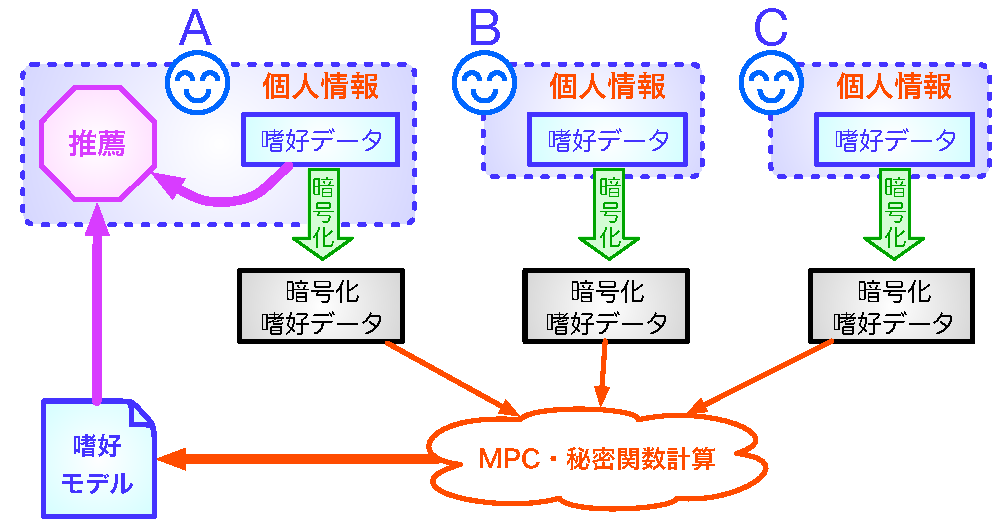
\includegraphics[width=0.96\fullwidth]{privacycf1.pdf}\\\smallskip
(a)~暗号化による方法\\\bigskip
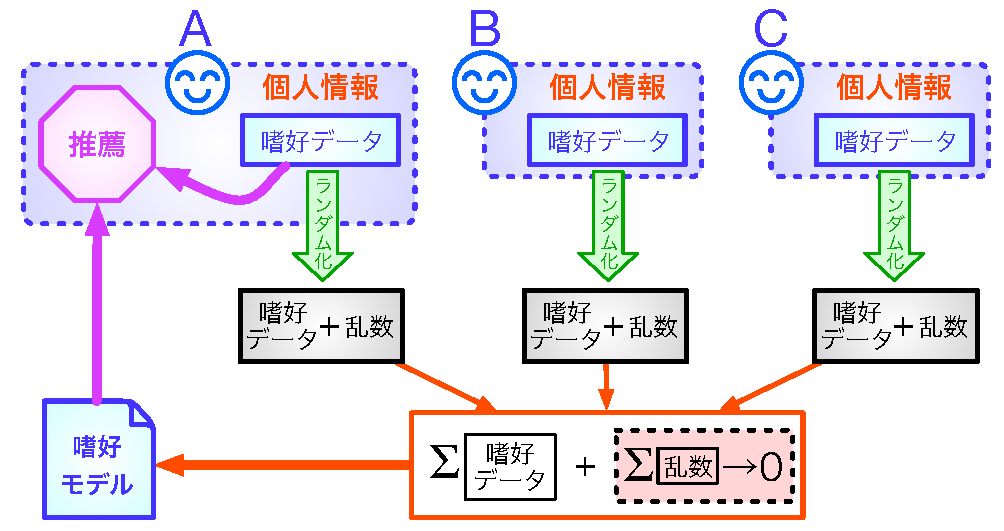
\includegraphics[width=0.96\fullwidth]{privacycf2.pdf}\\\smallskip
(b)ランダム化による方法
\caption{プライバシー保護協調フィルタリング}
\label{fig:privacycf}
\end{figure}

\section{暗号化による方法}

モデルベースの協調フィルタリングでは,標本利用者の嗜好データではなく,それらの規則性を表したモデルさえあれば推薦が可能である.
よって,嗜好データそのものを知らせることなくモデルが構築できれば,各利用者がどのような評価をしたかは秘匿できる.
また,メモリベースの協調フィルタリングでも,評価値行列を次元削減したものを公開すれば,個々のアイテムへの評価値は秘匿できる.
これを,データを暗号化したまま計算するという技術によって実現する.
この技術としては,ほとんどの計算が可能だが計算量は多い multiparty secure computation~\cite{misc:010}や,計算の種類ごとに専用の方法が必要だが高速に計算できる\term{秘密関数計算}{secure function evaluation}~\cite{kdde:02:03}がある.
\index{secure multiparty computation}

このアイデアに基づく枠組みを\ref{fig:privacycf}(a)に示す.
まず,標本利用者は自身の嗜好データを暗号化して推薦システムに渡す.
ここで,渡されたデータは暗号化されているため,個人情報は外部には漏れない.
これらの暗号化嗜好データに,秘密関数計算などの技術を適用して,暗号化された状態のモデルを獲得する.
最後に暗号化モデルを復号して目的の嗜好モデルを得る.
ここで,この嗜好モデルは標本利用者全般の嗜好の規則性の情報を表してはいるが,このモデルから個々の標本利用者の嗜好データ自体を復元することはできない.
よって,個人の評価情報は漏洩しない.
活動利用者は,自身の計算機上で,このモデルと自身の嗜好データから推薦を得ることができる.
モデルには,利用者間型メモリベースで次元縮約を使うもの\cite{ec:007}や,\ref{sec:funcmodel}の行列分解を使うもの\cite{sigir:02:01}などがある.

しかし,現状のプライバシー保護協調フィルタリングでは,社会的手段が補助的に必要となる.
計算結果が改竄されていないかを検証するには,半数以上の参加者は,個人情報を明かすほど信頼はできないが,計算の手続きは遵守する程度には信頼できるという semi-honest という前提が必要である.
しかし,この前提の技術的手段による保証は難しく,社会的手段によって保証しなければならない.
そのため,匿名で参加できるpeer-to-peerネットワークなどでの実現は難しい.
ソーシャル・ネットワークなど個人認証がなされるサービスでの推薦や,複数の企業が自身の顧客の情報を秘匿しつつ,共同して推薦をしたい場合などを想定すべきである.

\section{ランダム化による方法}

安全な計算は,暗号化はしているが,個人情報の真の値を外部に出している.
そうではなく,真の値ではない値を外部に出す方法が\term{ランダム化}{randomization}による方法(\ref{fig:privacycf}(b))である.

原理は単純で,平均値が0の正規分布や一様分布に従う乱数を加えてから,自分のデータを外部に出力する.
このとき,全参加者は同じ確率分布から独立にサンプリングした乱数を用いることが重要である.
ここで,全参加者の出力した値の総和や内積を求める.この値は,真の値の総和に,乱数の総和を加えたものになっている.
ここで乱数の総和は,元の分布の平均である$0$に漸近的に近づく.
よって,十分な数のデータがあれば,総和や内積が近似的に計算できる.
この手法によるプライバシー保護協調フィルタリングは\cite{icdm:03:01}などで提案されている.
この方法は,真の値は外部に出さなくて済む利点があるが,加える乱数の標準偏差が小さいと,真の値が近似的に予測できてしまうとか,厳密な値ではなく,近似値しか計算できないといった欠点がある.
